\chapter{Implementation}
\label{chap:impl}

\section{Navigation}

This chapter details the practical realization of the Automatic Learner Support (ALS) system, the comprehensive design of which was presented in Chapter \ref{chap:met}. The primary objective of the implementation phase was to translate the conceptual architecture and component logic into a functional software prototype capable of processing user conversations from the NamazApp e-learning application.
Section \ref{sec:als_implementation} describes the core ALS system. Then it elaborates on the step-by-step implementation of the ALS RAG pipeline itself, covering three iterative versions and all their stages.
Subsequently, in the chapter we focus on the development of the supplementary IslamQA Knowledge Base. Finally, the chapter summarizes the key implementation efforts.

\section{Automated Learner Support system}
\label{sec:als_implementation}

\subsection{Development stack}

We implemented the ALS system using a modern technology stack that was chosen considering its ease of integration, cost, and our expertise.

\subsubsection{Programming language and key libraries}

The programming language we use is Python version 3.12. As stated on the official website, “Python is a programming language that lets you work more quickly and integrate your systems more effectively” \cite{pythonwebsite}.
Key libraries we use include:
\begin{itemize}
    \item \textbf{Google Generative AI SDK (`google-genai`):} \cite{googlegenai} was the primary interface for all interactions with Google's Gemini Large Language Models (LLMs), used for both question extraction and answer generation.
    \item \textbf{Pandas (`pandas`):} \cite{pandas} was utilized for data manipulation tasks and for collecting the results in csv files for further results analysis.
    \item \textbf{HTTP Requests (`requests`):} \cite{requests} facilitated communication with external REST APIs, specifically the NamazApp Backend API for PAQ and IslamQA relevant fatawa retrieval and conversations dispatch.
    \item \textbf{JSON Handling (`json`):} \cite{json} was used for serializing and deserializing JSON data, which is the primary format for LLM inputs/outputs and API communications.
    \item \textbf{Pydantic (`pydantic`):} \cite{pydantic} was employed to make the code more structured and readable, define and validate the structure of data objects, especially for the expected JSON schemas from LLM responses and API payloads, ensuring data integrity throughout the pipeline.
\end{itemize}

\subsubsection{Large-language model}

The ALS system is based on Google's Gemini Flash 2.0 model \cite{gemini_flash_2} which was accessed via `google-genai` python library. This model is exploited for both unanswered questions retrieval and answer generation. The selection of this model was mainly driven by its cost-efficiency, which is crucial since the project has a limited budget. Furthermore, it has strong instruction-following capabilities, especially for answering in a specified json format, generating an answer only based on the provided sources. Moreover, it has a wide support of Russian and English languages, which are the primarily used languages in the project.

\subsection{Implementation of ALS RAG-pipeline}

To have fine-grained control over the system, we designed ALS as a pipeline that runs periodically (every hour). It is a Python script, more specifically a set of functions that are executed sequentially. We have not used any external libraries to create the RAG pipeline to avoid complicating the code. As we mentioned earlier, the pipeline processes active conversations. Each run processes 10 active conversations. This allows us to control ALS responses and provide a good user experience for mobile app users. The pipeline runs periodically as a cron job in a docker container on a server.

The implementation process was iterative: we implemented 3 versions of the pipeline and compared their results (see Chapter \ref{chap:eval}). We will discuss them in next sections; they are referred as versions v1, v2, and v3 respectively.
Further we will discuss the main pipeline steps in detail.

\subsubsection{Pulling active conversations}

The pipeline starts by fetching 10 active conversations from the NamazApp system. An active conversation is defined as a dialogue between a user and the expert in which the most recent message is from a user, and the conversation has not yet been marked as resolved. This process is handled by querying an API endpoint on the NamazApp Backend, which returns a list of conversations.

The following steps are applied to each of the retrieved active conversations sequentially.

\subsubsection{Questions and Salam extraction}

This step exploits the LLM to analyze and extract unanswered questions and salam from an active conversation. After analyzing the results of the v1 pipeline, we encountered an issue in this stage. So we decided to create the second version with the enhanced prompt for the question extraction. You can find the v1 prompt in Appendix~\ref{appex:prompt_for_extraction_v1}. And in Appendix~\ref{appex:prompt_for_extraction} the v2 prompt for this task is presented. 

The prompt utilizes several prompt engineering techniques to guide the Large Language Model (LLM) in distinguishing between answered and unanswered questions and handle diverse conversational patterns like question aggregation. This approach was reinforced in v2 by explicit negative constraints and strong directives against extracting already answered questions, a critical failure mode. Clear role definition ("structured user support chat processor"), precise task instructions, and strict JSON output formatting requirements were also key techniques used to maximize extraction accuracy and ensure reliable structured data for subsequent pipeline stages.

\subsubsection{Retrieve relevant documents (PAQs and IslamQA fatawa)}

For each unique unanswered question extracted in the previous step, the system attempts to find relevant information from its configured Knowledge Base. This involves querying two distinct sources: PAQs and IslamQA knowledge bases. The first two versions of the pipeline extracted and used only PAQs, and the IslamQA knowledge base was added in the v3 pipeline. It is performed via NamazApp backend that returns a list of the most semantically similar Previously Answered Questions (PAQs) and IslamQA fatawa along with their similarity scores.
Both sets of retrieved documents (PAQs and IslamQA chunks) are then passed through a filtering stage where only those exceeding a predefined similarity threshold are considered "accepted" for the subsequent answer generation step.

\subsubsection{Answer using relevant PAQs}

If accepted PAQs are present, the LLM in this stage tries to answer the question based on them. The full prompt is presented in Appendix~\ref{appex:prompt_for_answer_generation_using_paqs}. Here we are also using prompt engineering techniques such as role definition, precise sequential task instructions, a critical failure mode, and strict JSON output.

\subsubsection{Answer using relevant IslamQa fatawa}

We added this stage in the version 3 of the pipeline, to overcome the limitation of small size of the PAQ database. If there are no accepted PAQs or the LLM could not answer based on them, in this stage it tries to answer the question using information from IslamQA knowledge base. In Appendix~\ref{appex:prompt_for_answer_generation_using_islamqa} you can find the complete prompt text for this stage. This prompt also utilizes the same techniques for prompt engineering.

\subsubsection{Answer using LLM's general knowledge}

If there are neither relevant PAQs nor relevant IslamQa fatawa, the LLM tries to generate answer based on its general knowledge without relying on any additional external sources. This step is actually a result of the previous two steps. Its main purpose is to provide a draft for the answer and help an expert to answer the question.

\subsubsection{Decision to send the answer}

The decision making logic is based on the previous steps. Since only the PAQ database is considered completely reliable (since all answers are created or verified by the expert), the answer is sent only if it is based on relevant PAQs. In any other case, it is not sent. The expert then verifies these answers and decides whether they could be sent or require refactoring.

% Fig. \ref{fig:use-case-diagram} shows the main functionality of the system and the interactions between actors. Fig. \ref{fig:activity-diagram} contains the question processing flow. Firstly, the user asks a question, then the agentic AI, based on the retrieved documents from knowledge base (previously answered questions, articles, fatawas, etc.), decides if it can answer the question automatically on its own. If yes, it generates the answer and sends it to the user, otherwise, it redirects the question to the human operator.


% \begin{figure}
%     \centering
%     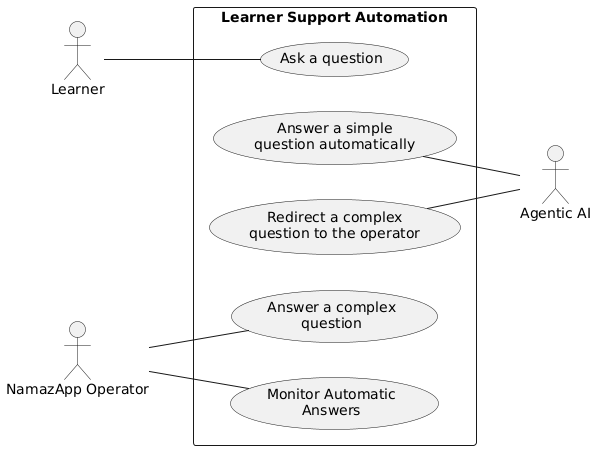
\includegraphics[width=0.5\linewidth]{figs/use_case_diagram.png}
%     \caption{Use-case diagram: a high-level overview of system functionality}
%     \label{fig:use-case-diagram}
% \end{figure}


\section{IslamQA Knowledge Base}
An essential part of our system is the knowledge database, which serves as the primary source of reference content for retrieval-augmented generation (RAG). This database contains domain-specific QA pairs, as well as structured information parsed from authentic Islamic resources. In this section, we describe our journey in selecting and implementing a suitable vector database solution, as well as the data preprocessing steps we undertake before populating the database.
\subsection{Suitable vector database}
\begin{enumerate}
    \item Initial Setup with Milvus:
    
    We first used Milvus, an open-source vector database, to store our embeddings. However, managing different tables for each resource was hard and not very flexible.

    \item Switching to Postgres with Vector Extension:
    
    To simplify things, we moved to PostgreSQL with a vector extension (like pgvector). This lets us store both text and vector data in one place, making our setup easier to manage.

    \item Deployment with Docker Compose:
    
    We containerized our database and services using Docker Compose. This approach made it simple to deploy and manage our entire system on the server.
\end{enumerate}

\subsection{Data preprocessing}
Before populating the database, we perform a series of preprocessing steps to ensure the data is clean, consistent, and readily searchable:
\begin{enumerate}
    \item Data Extraction:
    
    We gather content from various trusted Islamic sources like askimam.org,  askimam.ru, annisa-today.ru and etc.

    \item Parsing and Formatting:
    
    The data is cleaned and parsed into CSV files. This file contains text, metadata (like source and language), and unique IDs.
    
    
    \item Embedding Generation:
    
    For each text segment or QA pair, we generate a vector embedding using the OpenAI API. This process transforms the textual data into numerical representations, capturing semantic information useful for similarity searches.
    
    \item Inserting into the Database:
    
    Finally, we insert the text, metadata, and vector embeddings into our Postgres database. An index on the vector column helps us quickly find relevant data during searches.
\end{enumerate}

\section{Conclusion}

This chapter has detailed the practical implementation of the Automatic Learner Support (ALS) system, translating the design outlined in Chapter \ref{chap:met} into a functional prototype. Firstly, we have described the technology stack, then the specific implementation of all three versions of the core RAG pipeline components was elaborated. The crucial decision-making process for autonomously sending answers, which prioritizes reliability by only sending answers based exclusively on PAQs, was also detailed.
Furthermore, the chapter outlined the development of the IslamQA Knowledge Base, covering the selection and setup of a PostgreSQL database with vector extensions and the multi-step data preprocessing. The implementation choices, such as processing conversations in controlled batches and deploying the system as a cron job within a Docker container, were made to ensure manageable operation and a good user experience.
In the next chapter we will describe and discuss the collection and evaluation of results.
